\documentclass[aspectratio=169]{beamer}

\usepackage[utf8]{inputenc}
\usepackage[T1]{fontenc}
\usepackage{amsmath}
\usepackage{braket} % quantum notation
\usepackage{tcolorbox} % customization of boxes

\usepackage[T1]{fontenc}         % Not always necessary, but recommended.
% End of standard header.  What follows pertains to the problem at hand.

\usepackage{xcolor}
\usepackage{graphicx}
\usepackage{adjustbox}
\usepackage{mathtools}

\usepackage{tikz}
\usetikzlibrary{tikzmark,positioning,automata}
\usetikzlibrary{shapes.geometric}
\tikzstyle{every picture}+=[remember picture]

\usetheme{CambridgeUS}
\usecolortheme{rose}

\ProvidesPackage{mymacros}[2011/02/23 v1.0 My own macros]

\title[Quantum Computing: Grover's]{Quantum Computing}
\subtitle{A Gentle Introduction to Grover's Algorithm}

\immediate\write18{echo $VERSION > version.tex}
\date{\today\\ v1.0
}
\author[jmaunon]{Juan Miguel Au\~n\'on Garc\'ia}
\newcount\colveccount
\newcommand*\colvec[1]{
        \global\colveccount#1
        \begin{pmatrix}
        \colvecnext
}
\def\colvecnext#1{
        #1
        \global\advance\colveccount-1
        \ifnum\colveccount>0
                \\
                \expandafter\colvecnext
        \else
                \end{pmatrix}
        \fi
}


%%%%%%%%%%%%% TIKZ

\tikzset{
	invisible/.style={opacity=0,text opacity=0},
	visible on/.style={alt=#1{}{invisible}},
	alt/.code args={<#1>#2#3}{%
		\alt<#1>{\pgfkeysalso{#2}}{\pgfkeysalso{#3}} 
	},
}

\tikzset{
	background fill/.style={fill=#1},
	background fill/.default={white},
	fill on/.style={alt=#1{}{background fill}},
}

\tikzset{
	background draw/.style={draw=#1},
	background draw/.default={white},
	draw on/.style={alt=#1{}{background draw}},
}

\tikzset{
	background filldraw/.style 2 args={draw=#1, fill=#2},
	background filldraw/.default={white}{white},
	filldraw on/.style={alt=#1{}{background filldraw}},
}

\tikzset{
	background shade/.style={#1},
	background shade/.default={top color=white, bottom color=white},
	shade on/.style={alt=#1{}{background shade}},
}

\tikzset{
	background shadedraw/.style 2 args={draw=#1, #2},
	background shadedraw/.default={white}{top color=white, bottom color=white},
	shadedraw on/.style={alt=#1{}{background shadedraw}},
}

\tikzset{onslide/.code args={<#1>#2}{%
		\only<#1>{\pgfkeysalso{#2}}
	}}


% These options will be applied to all `tcolorboxes`
\tcbset{%
    noparskip,
    colback=gray!10, %background color of the box
    colframe=gray!40, %color of frame and title background
    coltext=black, %color of body text
    coltitle=black, %color of title text 
    fonttitle=\bfseries,
    alerted/.style={coltitle=black, 
                     colframe=blue!70},
    example/.style={coltitle=black, 
                     colframe=blue!90},
    }

%===== custom toc =====
\setbeamertemplate{section in toc}{%
	{\color{orange!70!black}\inserttocsectionnumber.}~\inserttocsection}
\setbeamercolor{subsection in toc}{bg=white,fg=structure}
\setbeamertemplate{subsection in toc}{%
	\hspace{1.2em}{\color{orange}\inserttocsectionnumber.\inserttocsubsectionnumber.}~\inserttocsubsection\par}

%===== custom toc at begin section/subsection =====
\newif\ifshowtoc
\showtoctrue
\AtBeginSection{%
\ifshowtoc
{\setbeamercolor{background canvas}{bg=white}
\begin{frame}[plain]
\frametitle{Outline}

\tableofcontents[currentsection]
\end{frame}}
\fi
}

\newif\ifshowtoc
\showtoctrue
\AtBeginSubsection{%
	\ifshowtoc
	{\setbeamercolor{background canvas}{bg=white}
		\begin{frame}[plain]
			\frametitle{Outline}
						
			\tableofcontents[ currentsection,
			currentsubsection,
			subsectionstyle=show/shaded]
	\end{frame}}
	\fi
}

%===== custom headline =====

\setbeamertemplate{headline}{%

	\begin{beamercolorbox}[ht=2.5ex]{section in head/foot}
		%\vskip2pt\insertnavigation{\paperwidth}\vskip2pt
		\vskip2pt\insertsectionnavigationhorizontal{\paperwidth}{}{\hskip0pt plus1filll}
	\end{beamercolorbox}%
	%   \ifbeamer@theme@subsection%

	\begin{beamercolorbox}[ht=2.5ex,dp=1.125ex,%
		leftskip=.3cm,rightskip=.3cm plus1fil]{subsection in head/foot}
		\vskip2pt\insertsubsectionnavigationhorizontal{\paperwidth}{}{\hskip0pt plus1filll}
	\end{beamercolorbox}%

}

% Default fixed font does not support bold face
\DeclareFixedFont{\ttb}{T1}{txtt}{bx}{n}{12} % for bold
\DeclareFixedFont{\ttm}{T1}{txtt}{m}{n}{12}  % for normal

% Custom colors
\usepackage{color}
\definecolor{deepblue}{rgb}{0,0,0.5}
\definecolor{deepred}{rgb}{0.6,0,0}
\definecolor{deepgreen}{rgb}{0,0.5,0}

\usepackage{listings}

% Python style for highlighting
\newcommand\pythonstyle{\lstset{
language=Python,
basicstyle=\ttm,
otherkeywords={self},             % Add keywords here
keywordstyle=\ttb\color{deepblue},
emph={MyClass,__init__},          % Custom highlighting
emphstyle=\ttb\color{deepred},    % Custom highlighting style
stringstyle=\color{deepgreen},
frame=tb,                         % Any extra options here
showstringspaces=false            % 
}}


% Python environment
\lstnewenvironment{python}[1][]
{
\pythonstyle
\lstset{#1}
}
{}

% Python for external files
\newcommand\pythonexternal[2][]{{
\pythonstyle
\lstinputlisting[#1]{#2}}}

% Python for inline
\newcommand\pythoninline[1]{{\pythonstyle\lstinline!#1!}}

\begin{document}

\begin{frame}
\titlepage
\end{frame}

\begin{frame}[plain]
\frametitle{Outline}
\tableofcontents
\end{frame}

\section{Grover's algorithm}
\subsection{Motivation \& Outline}
\begin{frame}
\frametitle{Grover's algorithm: Motivation}
Grover's algorithm performs a search over an unorder set of $2^n$ items fo find the unique element that satisfies some condition

\end{frame}
\begin{frame}
	\frametitle{Grover's algorithm: Outline}
	\begin{tikzpicture}[
	expl/.style={draw=black, thick=2pt,fill=blue!20,rounded corners},
	arrow/.style={red!80!black,ultra thick,->,>=latex}]	
	\node[anchor=south west,inner sep=0] (image) at (0,0) {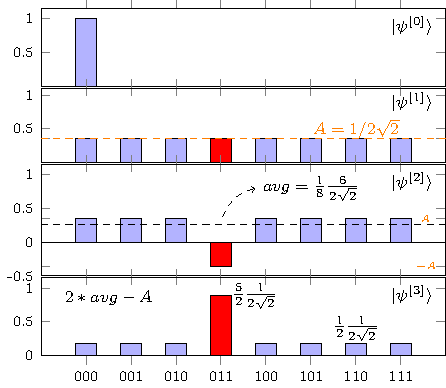
\includegraphics[width=0.5\textwidth]{figures/bar-graph/probs.pdf}};
	\begin{scope}[x={(image.south east)},y={(image.north west)}]
		%\draw[help lines,xstep=.1,ystep=.1] (0,0) grid (1,1);
		%\foreach \x in {0,1,...,9} { \node [anchor=north] at (\x/10,0) {0.\x}; }
		%\foreach \y in {0,1,...,9} { \node [anchor=east] at (0,\y/10) {0.\y}; }
		\node[expl](A) at (1.5,0.875) {\Large Initial state $\ket{\psi^{[0]}}$};
		\node[expl](B) at (1.5,0.65) {\Large Initialization $\ket{\psi^{[1]}}$};
		\node[expl](C) at (1.5,0.4) {\Large Sign flip $\ket{\psi^{[2]}}$};
		\node[expl](D) at (1.5,0.15) {\Large Inversion about average $\ket{\psi^{[3]}}$};
		
		\draw[arrow] (A.south) -- node [right]{Hadamard $H$} (B.north);
		\draw[arrow] (B.south) -- node [right]{Oracle $U_f$} (C.north);
		\draw[arrow] (C.south) -- node [right]{Difussion $U_d$} (D.north);
		\draw[arrow] (D.north east) to[bend right] node [right]{$\frac{\pi}{4}\sqrt{n}$} (B.east);
	\end{scope}

	\end{tikzpicture}	
\end{frame}

\subsection{Steps}
\begin{frame}
	\frametitle{Initialization}
	\begin{tikzpicture}[
	expl/.style={draw=black, thick=2pt,fill=blue!20,rounded corners},
	arrow/.style={red!80!black,ultra thick,->,>=latex}]	
	\node[anchor=south west,inner sep=0] (image) at (0,0) {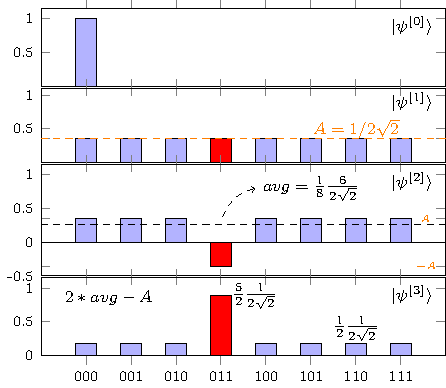
\includegraphics[width=0.5\textwidth]{figures/bar-graph/probs.pdf}};
	\begin{scope}[x={(image.south east)},y={(image.north west)}]
	%\draw[help lines,xstep=.1,ystep=.1] (0,0) grid (1,1);
	%\foreach \x in {0,1,...,9} { \node [anchor=north] at (\x/10,0) {0.\x}; }
	%\foreach \y in {0,1,...,9} { \node [anchor=east] at (0,\y/10) {0.\y}; }
	\node[expl](A) at (1.5,0.875) {\Large Initial state $\ket{\psi^{[0]}}$};
	\node[expl](B) at (1.5,0.65) {\Large Initialization $\ket{\psi^{[1]}}$};
	\node[expl](C) at (1.5,0.4) {\Large Sign flip $\ket{\psi^{[2]}}$};
	\node[expl](D) at (1.5,0.15) {\Large Inversion about average $\ket{\psi^{[3]}}$};
	
	\draw[arrow] (A.south) -- node [right]{Hadamard $H$} (B.north);
	\draw[arrow] (B.south) -- node [right]{Oracle $U_f$} (C.north);
	\draw[arrow] (C.south) -- node [right]{Difussion $U_d$} (D.north);
	\draw[thick,dashed] (0.01,0.575) rectangle (1.85,1);
	\draw[arrow] (D.north east) to[bend right] node [right]{$\frac{\pi}{4}\sqrt{n}$} (B.east);
	\end{scope}
	
	\end{tikzpicture}	
\end{frame}
\begin{frame}
\frametitle{Initialization}
We find a method (unitary operator) to have all the states with the same probability (\textit{principle of superposition}). 
\pause
\begin{eqnarray}
(I^{\otimes n}\otimes X)\left.|0\right\rangle _{n+1}&=&\left.|0\right\rangle _{n}\otimes\left.|1\right\rangle \nonumber\\
H^{\otimes\left(n+1\right)}\left[(I^{\otimes n}\otimes X)\left.|0\right\rangle _{n+1}\right]&=&H^{\otimes n}\left.|0\right\rangle _{n}\otimes H\left.|1\right\rangle \nonumber\\
&=&\sum_{j\in\{0,1\}^{n}}\frac{1}{\sqrt{2^{n}}}\left.|j\right\rangle _{n}\otimes\frac{1}{\sqrt{2}}\left(\left.|0\right\rangle -\left.|1\right\rangle \right)\nonumber\\
&=&\sum_{j\in\{0,1\}^{n}}\alpha_{j}\left.|j\right\rangle _{n}\otimes\frac{1}{\sqrt{2}}\left(\left.|0\right\rangle -\left.|1\right\rangle \right)\nonumber\\
&=&\ket{\psi^{[1]}}\nonumber
\end{eqnarray}
\end{frame}

\begin{frame}
\frametitle{Initialization}

\begin{exampleblock}{3-qubit example: Set ancillary qubit to $\ket{1}$}
\begin{eqnarray}
(I^{\otimes3}\otimes X)\left.|0\right\rangle _{3+1}&=&I^{\otimes3}\left.|0\right\rangle _{3}\otimes X\left.|0\right\rangle \nonumber\\
&=&\begin{pmatrix*}[c]
1&0&0&0&0&0&0&0\\
0&1&0&0&0&0&0&0\\
0&0&1&0&0&0&0&0\\
0&0&0&1&0&0&0&0\\
0&0&0&0&1&0&0&0\\
0&0&0&0&0&1&0&0\\
0&0&0&0&0&0&1&0\\
0&0&0&0&0&0&0&1\\
\end{pmatrix*}\left(\begin{array}{c}
1\\
0\\
0\\
0\\
0\\
0\\
0\\
0
\end{array}\right)\otimes\left(\begin{array}{cc}
0 & 1\\
1 & 0
\end{array}\right)\left(\begin{array}{c}
1\\
0
\end{array}\right)\nonumber\\
&=&\left.|0\right\rangle_3 \otimes\left.|1\right\rangle \nonumber
\end{eqnarray}
\end{exampleblock}


\end{frame}

\begin{frame}
\frametitle{Initialization}
\begin{exampleblock}{3-qubit example: Apply Hadamard gate}
\begin{eqnarray}
\ket{\psi^{[1]}}&=&H^{\otimes\left(3+1\right)}\left[(I^{\otimes3}\otimes X)\left.|0\right\rangle _{n+1}\right]\nonumber\\
&=&H^{\otimes3}\left.|0\right\rangle_3 \otimes H\left.|1\right\rangle\nonumber\\
&=&\frac{1}{\sqrt{2^{3}}}\begin{pmatrix*}[r]
1 & 1 & 1 & 1 & 1 & 1 & 1 & 1\\
1 & -1 & 1 & -1 & 1 & -1 & 1 & -1\\
1 & 1 & -1 & -1 & 1 & 1 & -1 & -1\\
1 & -1 & -1 & 1 & 1 & -1 & -1 & 1\\
1 & 1 & 1 & 1 & -1 & -1 & -1 & -1\\
1 & -1 & 1 & -1 & -1 & 1 & -1 & 1\\
1 & 1 & -1 & -1 & -1 & -1 & 1 & 1\\
1 & -1 & -1 & 1 & -1 & 1 & 1 & -1
\end{pmatrix*}\left(\begin{array}{c}
1\\
0\\
0\\
0\\
0\\
0\\
0\\
0
\end{array}\right)\otimes\frac{1}{\sqrt{2}}\left(\begin{array}{cc}
1 & 1\\
1 & -1
\end{array}\right)\left(\begin{array}{c}
0\\
1
\end{array}\right)\nonumber
\end{eqnarray}
\end{exampleblock}
\end{frame}

\begin{frame}
	\frametitle{Initialization}
	\begin{exampleblock}{3-qubit example: Apply Hadamard gate}
		\begin{eqnarray}
			\ket{\psi^{[1]} }&=&\frac{1}{\sqrt{2^{3}}}\begin{pmatrix*}
			1 1 1 1 1 1 1 1
			\end{pmatrix*}^{\dagger}\otimes\frac{1}{\sqrt{2}}\left(\begin{array}{c}
			1\\
			-1
			\end{array}\right)\nonumber\\
			&=&[ \frac{1}{2\sqrt{2}}\left.|000\right\rangle +\frac{1}{2\sqrt{2}}\left.|001\right\rangle +\frac{1}{2\sqrt{2}}\left.|010\right\rangle +\frac{1}{2\sqrt{2}}\left.|011\right\rangle \nonumber\\
			&+&\frac{1}{2\sqrt{2}}\left.|100\right\rangle +\frac{1}{2\sqrt{2}}\left.|101\right\rangle +\frac{1}{2\sqrt{2}}\left.|110\right\rangle +\frac{1}{2\sqrt{2}}\left.|111\right\rangle] \nonumber\\
			&\otimes&\frac{1}{\sqrt{2}}\left(\left.|0\right\rangle -\left.|1\right\rangle \right)		\nonumber	
		\end{eqnarray}
	\end{exampleblock}
\end{frame}

\begin{frame}{}
	\frametitle{Initialization}
	\begin{exampleblock}{3-qubit example: Summary}
		\begin{eqnarray}
			\ket{\psi^{[1]} }&=&
			H^{\otimes\left(3+1\right)}\left[(I^{\otimes3}\otimes X)\left.|0\right\rangle _{n+1}\right]\nonumber\\
			&=&[\frac{1}{2\sqrt{2}}\left.|000\right\rangle +\frac{1}{2\sqrt{2}}\left.|001\right\rangle +\frac{1}{2\sqrt{2}}\left.|010\right\rangle +\frac{1}{2\sqrt{2}}\left.|011\right\rangle\nonumber\\ &+&\frac{1}{2\sqrt{2}}\left.|100\right\rangle +\frac{1}{2\sqrt{2}}\left.|101\right\rangle +\frac{1}{2\sqrt{2}}\left.|110\right\rangle +\frac{1}{2\sqrt{2}}\left.|111\right\rangle ]\nonumber\\
			&\otimes&\frac{1}{\sqrt{2}}\left(\left.|0\right\rangle -\left.|1\right\rangle \right)\nonumber\\
			&=&\sum_{j\in\{0,1\}^{n}}\frac{1}{\sqrt{2^{n}}}\left.|j\right\rangle _{n}\otimes\frac{1}{\sqrt{2}}\left(\left.|0\right\rangle -\left.|1\right\rangle \right)=\ket{\psi^{[1]} }\nonumber
		\end{eqnarray}
	\end{exampleblock}
\end{frame}



\begin{frame}
	\frametitle{Sign flip}
	\begin{tikzpicture}[
	expl/.style={draw=black, thick=2pt,fill=blue!20,rounded corners},
	arrow/.style={red!80!black,ultra thick,->,>=latex}]	
	\node[anchor=south west,inner sep=0] (image) at (0,0) {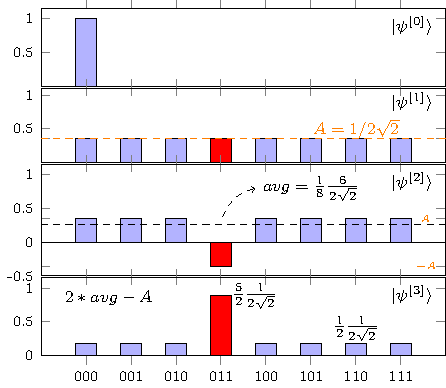
\includegraphics[width=0.5\textwidth]{figures/bar-graph/probs.pdf}};
	\begin{scope}[x={(image.south east)},y={(image.north west)}]
	%\draw[help lines,xstep=.1,ystep=.1] (0,0) grid (1,1);
	%\foreach \x in {0,1,...,9} { \node [anchor=north] at (\x/10,0) {0.\x}; }
	%\foreach \y in {0,1,...,9} { \node [anchor=east] at (0,\y/10) {0.\y}; }
	\node[expl](A) at (1.5,0.875) {\Large Initial state $\ket{\psi^{[0]}}$};
	\node[expl](B) at (1.5,0.65) {\Large Initialization $\ket{\psi^{[1]}}$};
	\node[expl](C) at (1.5,0.4) {\Large Sign flip $\ket{\psi^{[2]}}$};
	\node[expl](D) at (1.5,0.15) {\Large Inversion about average $\ket{\psi^{[3]}}$};
	
	\draw[arrow] (A.south) -- node [right]{Hadamard $H$} (B.north);
	\draw[arrow] (B.south) -- node [right]{Oracle $U_f$} (C.north);
	\draw[arrow] (C.south) -- node [right]{Difussion $U_d$} (D.north);
	\draw[thick,dashed] (0.01,0.3) rectangle (1.85,0.75);
	\draw[arrow] (D.north east) to[bend right] node [right]{$\frac{\pi}{4}\sqrt{n}$} (B.east);
	\end{scope}	
	\end{tikzpicture}	
\end{frame}
\begin{frame}
	\frametitle{Sign flip}
	We find a method (unitary operator) which flip the sign of the state of interest.
	\pause
	\begin{block}{\textit{Quantum Oracle}}
		It is defined the operator $U_f$: 
		\[U_{f}:\left.|j\right\rangle _{n}\otimes\left.|y\right\rangle _{1}\rightarrow\left.|j\right\rangle _{n}\otimes\left.|y\oplus f\left(j\right)\right\rangle _{1},\]
		where $\oplus$ is the sum operator in mod 2, and $f\left(j\right)=\left\{ \begin{array}{cc}
		1  & j=l\\
		0  & j\neq l
		\end{array}\right\} $
	\end{block}
	
	
	\begin{center}
		\begin{tabular}{|c c |c|} 
			\hline
			A & B & XOR \\ 
			\hline\hline
			0&0&0  \\ 
			\hline
			0&1&1  \\ 
			\hline
			1&0&1  \\
			\hline
			1&1&0 \\
			\hline
		\end{tabular}
	\end{center}
\end{frame}

\begin{frame}
	\frametitle{Sign flip}
	We apply $U_f$ (\textit{Quantum Oracle}) to the previous state $\psi^{[1]}$
	\begin{eqnarray}
		\ket{\psi^{[2]}}&=& U_{f}\ket{\psi^{[1]}}\nonumber\\
			&=&U_{f}\left(\sum_{j\in\{0,1\}^{n}}\alpha_{j}\left.|j\right\rangle _{n}\otimes\frac{1}{\sqrt{2}}\left(\left.|0\right\rangle -\left.|1\right\rangle \right)\right)\nonumber\\
		&=&U_{f}\left(\alpha_{l}\left.|l\right\rangle _{n}\otimes\frac{1}{\sqrt{2}}\left(\left.|0\right\rangle -\left.|1\right\rangle \right)+\sum_{
			j\in\{0,1\}^{n};\;
			j\neq l
			}\alpha_{j}\left.|j\right\rangle _{n}\otimes\frac{1}{\sqrt{2}}\left(\left.|0\right\rangle -\left.|1\right\rangle \right)\right)\nonumber\\
		&=&\left(\tikz[baseline]{
			\node[fill=blue!20,anchor=base, fill on=<2->,draw=red,rounded corners,draw on =<3>] (A)
			{$ -\alpha_{l}\left.|l\right\rangle _{n}$};
		} 
				 +\sum_{j\in\{0,1\}^{n};\;
				 	j\neq l}\alpha_{j}\left.|j\right\rangle _{n}\right)\otimes\tikz[baseline]{
			\node[fill=blue!20,anchor=base, fill on=<3>,draw=red,draw on =<3>,rounded corners] (AA)
			{$ \frac{1}{\sqrt{2}}\left(\left.|0\right\rangle -\left.|1\right\rangle \right)$};\nonumber
		} 
	\end{eqnarray}
	\begin{tikzpicture}[
	remember picture,
	overlay,
	expl/.style={draw=red, thick=2pt,fill=blue!20,rounded corners},
	arrow/.style={red!80!black,ultra thick,->,>=latex}
	]
	\onslide<2->{\node[expl, xshift = -3cm](B) at (current page.center) {\Large sign flip!};}
	\onslide<2->{\draw[arrow]
	(A.north) to[bend left] (B.south);}
	\onslide<3->{\node[expl, xshift = 3cm](BB) at (current page.center) {\Large Extra qubit!};}
	\onslide<3->{\draw[arrow]
		(AA.north) to[bend right] (BB.south);}
	\end{tikzpicture}
\end{frame}


\begin{frame}
	\frametitle{Sign flip\footnote{This slide shows the result of applying $U_f$ but not how is applied. This is because this step of the algorithm depends on the specific problem.}}
	\begin{exampleblock}{3-qubit example: Quantum Oracle}
		\begin{eqnarray}		
		\ket{\psi^{[2]}} &=& U_f\ket{\psi^{[1]}} \nonumber\\
		&=&[\frac{1}{2\sqrt{2}}\left.|000\right\rangle +\frac{1}{2\sqrt{2}}\left.|001\right\rangle +\frac{1}{2\sqrt{2}}\left.|010\right\rangle -\frac{1}{2\sqrt{2}}\left.|011\right\rangle\nonumber\\ &+&\frac{1}{2\sqrt{2}}\left.|100\right\rangle +\frac{1}{2\sqrt{2}}\left.|101\right\rangle +\frac{1}{2\sqrt{2}}\left.|110\right\rangle +\frac{1}{2\sqrt{2}}\left.|111\right\rangle ]\nonumber\\
		&\otimes&\frac{1}{\sqrt{2}}\left(\left.|0\right\rangle -\left.|1\right\rangle \right)\nonumber
		\end{eqnarray}
	\end{exampleblock}
\end{frame}

\begin{frame}
	\frametitle{Inversión con con respecto la media}
	Buscamos una forma (operador unitario) de invertir el valor de la amplitud con respecto la media.
	\begin{equation*}
		\sum_{j\in\{0,1\}^{n}}\alpha_{j}\left.|j\right\rangle _{n}\stackrel{U_d}{\longrightarrow}\sum_{j\in\{0,1\}^{n}}\left(2\left(\sum_{k\in\{0,1\}^{n}}\frac{\alpha_{k}}{2^{n}}\right)-\alpha_{j}\right)\left.|j\right\rangle _{n},
	\end{equation*}
	donde $\sum_{k\in\{0,1\}^{n}}\frac{\alpha_{k}}{2^{n}}$ es el valor medio.
	\begin{exampleblock}{}
		\[\sum_{k\in\{0,1\}^{n}}\frac{\alpha_{k}}{2^{n}}=\frac{1}{2^3}\frac{6}{2\sqrt{2}}\]
	\end{exampleblock}
\end{frame}
\begin{frame}
	\frametitle{Inversión con respecto la media}
	\begin{block}{\textit{Difussion operator }}
		\begin{eqnarray}
			U_{d}=\left(\begin{array}{cccc}
			\frac{2}{2^{n}} & \frac{2}{2^{n}} & \cdots & \frac{2}{2^{n}}\\
			\frac{2}{2^{n}} & \frac{2}{2^{n}} & \cdots & \frac{2}{2^{n}}\\
			\vdots & \vdots & \ddots & \vdots\\
			\frac{2}{2^{n}} & \frac{2}{2^{n}} & \cdots & \frac{2}{2^{n}}
			\end{array}\right)-I^{\otimes n}=\dots=-H^{\otimes n}DH^{\otimes n},
		\end{eqnarray}
		donde $D=diag\left(-1,1,1,\cdots,1\right)$
	\end{block}
\end{frame}

\begin{frame}[fragile]{}
	\frametitle{Inversion con respecto la media}
	\begin{exampleblock}{Difussion operator in python}
		\vspace*{0.5cm}
		\begin{adjustbox}{max width=0.9\textwidth}
			\begin{python}
>>> import numpy as np
>>> H1 = 1/np.sqrt(2)*np.array([[1,1],[1, -1]]) # Hadamard operator 1 qubit
>>> H2 = np.kron(H1,H1) # Hadamard operator 2 qubit
>>> H3 = np.kron(H2,H1) # Hadamard operator 3 qubit

>>> D = np.eye(8) # Diagonal operator
>>> D[0,0] = -1

>>> Ud = -np.dot(np.dot(H3,D),H3) # Difussion operator
>>> psi = 1/(2*np.sqrt(2))*np.array([1,1,1,-1,1,1,1,1]) # Initial state

>>> psi_2 = np.dot(Uw,psi)
>>> print(psi_2)
array([0.176 , 0.176 , 0.176 , 0.883, 0.176, 0.176, 0.176, 0.176])
			\end{python}
		\end{adjustbox}
	\end{exampleblock}

\end{frame}
\begin{frame}
	\frametitle{Inversión con respecto la media}
	\begin{exampleblock}{Difussion operator}
	\begin{eqnarray}
	U_d = -\frac{1}{8}\frac{1}{2\sqrt{2}}\begin{pmatrix*}[r]
	6 & -2 & -2 & -2 & -2 & -2 & -2 & -2\\
	-2 & 6 & -2 & -2 & -2 & -2 & -2 & -2\\
	-2 & -2 & 6 & -2 & -2 & -2 & -2 & -2\\
	-2 & -2 & -2 & 6 & -2 & -2 & -2 & -2\\
	-2 & -2 & -2 & -2 & 6 & -2 & -2 & -2\\
	-2 & -2 & -2 & -2 & -2 & 6 & -2 & -2\\
	-2 & -2 & -2 & -2 & -2 & -2 & 6 & -2\\
	-2 & -2 & -2 & -2 & -2 & -2 & -2 & 6
	\end{pmatrix*}
		\begin{pmatrix*}[r]
		1\\
		1\\
		1\\
		-1\\
		1\\
		1\\
		1\\
		1
		\end{pmatrix*}=\frac{1}{4\sqrt{2}}
		\left(
		\begin{tabular}{c}
		1\\
		1\\
		1\\
		5\\
		1\\
		1\\
		1\\
		1
		\end{tabular}
		\right)\nonumber
	\end{eqnarray}
	\end{exampleblock}
\end{frame}
\begin{frame}[t]
	\frametitle{Measurement \& Repetition}	
	For the first iteration we measure
		\[
		\boxed{
		\begin{array}{cccccccc}
			\alpha_{011} &=& \frac{5}{2}\frac{1}{2\sqrt{2}}&\longrightarrow& \left\| \alpha_{011}\right\|^2 &\simeq& 78,12\% &\\
			\alpha_{j} &=& \frac{1}{2}\frac{1}{2\sqrt{2}}&\longrightarrow& \left\| \alpha_{j}\right\|^2 &\simeq& 3,12\% & \left(j\neq \ket{011}\right)\\
		\end{array}
		}
		\]
	The optimal number of repetitions $R\simeq\frac{\pi}{4}\sqrt{n}\simeq 2.2$. 
	For the second iteration (Oracle $\&$ Diffusion) we have:
		 \[
		 \boxed{
		 	\begin{array}{cccccccc}
		 	\alpha_{011} &=& \frac{11}{4}\frac{1}{2\sqrt{2}}&\longrightarrow& \left\| \alpha_{011}\right\|^2 &\simeq& 94,5\% &\\
		 	\alpha_{j} &=& \frac{-1}{4}\frac{1}{2\sqrt{2}}&\longrightarrow& \left\| \alpha_{j}\right\|^2 &\simeq& 0,78\% & \left(j\neq \ket{011}\right)\\
		 	\end{array}
		 }
		\]
\end{frame}

\section{Implementation of Grover's algorithm: 2-Qubit States}
\subsection{Quantum Circuit}
\begin{frame}
	\frametitle{2-Qubit Quantum Circuit}
	\only<2>{\framesubtitle{Initialization}}
	\begin{tikzpicture}	
	\node[anchor=south west,inner sep=0] (image) at (0,0) {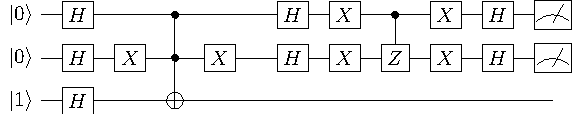
\includegraphics[width=0.9\textwidth]{figures/circuits/2-qubit.pdf}};
	\begin{scope}[x={(image.south east)},y={(image.north west)}]
		%\draw[help lines,xstep=.1,ystep=.1] (0,0) grid (1,1);
		%\foreach \x in {0,1,...,9} { \node [anchor=north] at (\x/10,0) {0.\x}; }
		%\foreach \y in {0,1,...,9} { \node [anchor=east] at (0,\y/10) {0.\y}; }
		\draw<2->[thick,dashed] (0.085,-0.05) rectangle (0.185,1.05);
		\node<2-> [above] at (0.125,1.1) {Initialization};
	\end{scope}

	\end{tikzpicture}	
\end{frame}

\begin{frame}
	\frametitle{2-Qubit Quantum Circuit}
	\framesubtitle{Initialization}
	\begin{eqnarray*}
		\psi^{[0]} & = & \ket{001}\\
		\psi^{[1]} & = & H^{\otimes 3} \psi^{[0]}\\
				   & = & \frac{1}{\sqrt{8}}\left(\ket{000} + \ket{010} + \ket{100} + \ket{110} - \left.\ket{001} - \ket{011} - \ket{101} - \ket{111} \right) \right.\\ 
	\end{eqnarray*}
\end{frame}

\begin{frame}
	\frametitle{2-Qubit Quantum Circuit}
	\framesubtitle{Quantum Oracle}
	\begin{tikzpicture}	
	\node[anchor=south west,inner sep=0] (image) at (0,0) {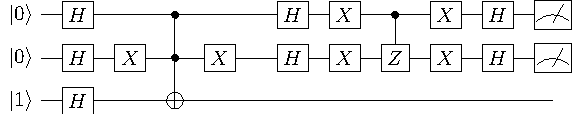
\includegraphics[width=0.9\textwidth]{figures/circuits/2-qubit.pdf}};
	\begin{scope}[x={(image.south east)},y={(image.north west)}]
	%\draw[help lines,xstep=.1,ystep=.1] (0,0) grid (1,1);
	%\foreach \x in {0,1,...,9} { \node [anchor=north] at (\x/10,0) {0.\x}; }
	%\foreach \y in {0,1,...,9} { \node [anchor=east] at (0,\y/10) {0.\y}; }
	\draw<1->[thick,dashed] (0.085,-0.05) rectangle (0.185,1.05);
	\node<1-> [above] at (0.125,1.1) {Initialization};
	
	\draw<1->[thick,dashed] (0.185,-0.05) rectangle (0.45,1.05);
	\node<1-> [above] at (0.3125,1.1) {Quantum Oracle};
	\end{scope}
	
	\end{tikzpicture}	
\end{frame}

\begin{frame}
	\frametitle{2-Qubit Quantum Circuit}
	\framesubtitle{Quantum Oracle}
	
	\begin{eqnarray*}
		U_f & = & \left(I\otimes X \otimes I\right) \cdot T \cdot \left(I\otimes X \otimes I\right) = 
			\begin{pmatrix*}[r]
					1 & 0 & 0 & 0 & 0 & 0 & 0 & 0 \\
					0 & 1 & 0 & 0 & 0 & 0 & 0 & 0 \\
					0 & 0 & 1 & 0 & 0 & 0 & 0 & 0 \\
					0 & 0 & 0 & 1 & 0 & 0 & 0 & 0 \\
					0 & 0 & 0 & 0 & 0 & 1 & 0 & 0 \\
					0 & 0 & 0 & 0 & 1 & 0 & 0 & 0 \\
					0 & 0 & 0 & 0 & 0 & 0 & 1 & 0 \\
					0 & 0 & 0 & 0 & 0 & 0 & 0 & 1
		    \end{pmatrix*}
	\end{eqnarray*}
\end{frame}

\begin{frame}
	\frametitle{2-Qubit Quantum Circuit}
	\framesubtitle{Quantum Oracle}
	
	\begin{eqnarray*}
		\psi^{[1]} & = &\frac{1}{\sqrt{8}}\left(\ket{000} + \ket{010} + \ket{100} + \ket{110} - \ket{001} - \ket{011} - \ket{101} - \ket{111} \right) \\  
		\psi^{[2]} & = & U_f\ket{\psi^{[1]}}\\
				   & = & \frac{1}{\sqrt{8}}\left(\ket{000} + \ket{010} + \ket{101} + \ket{110} - \ket{001} - \ket{011} - \ket{100} - \ket{111} \right) \\  
				   & = & \frac{1}{\sqrt{8}}\left(\ket{00} + \ket{01} - \ket{10} + \ket{11}\right)\otimes\left(\ket{0} - \ket{1}\right) \\
				   & = & \frac{1}{2}\left(\ket{00} + \ket{01} - \ket{10} + \ket{11}\right)\otimes\frac{1}{\sqrt{2}}\left(\ket{0} - \ket{1}\right)
	\end{eqnarray*}
\end{frame}

\begin{frame}
	\frametitle{2-Qubit Quantum Circuit}
	\framesubtitle{Difussion Operator}
	\begin{tikzpicture}	
	\node[anchor=south west,inner sep=0] (image) at (0,0) {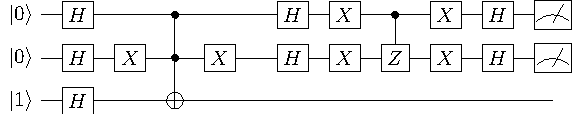
\includegraphics[width=0.9\textwidth]{figures/circuits/2-qubit.pdf}};
	\begin{scope}[x={(image.south east)},y={(image.north west)}]
	%\draw[help lines,xstep=.1,ystep=.1] (0,0) grid (1,1);
	%\foreach \x in {0,1,...,9} { \node [anchor=north] at (\x/10,0) {0.\x}; }
	%\foreach \y in {0,1,...,9} { \node [anchor=east] at (0,\y/10) {0.\y}; }
	\draw<1->[thick,dashed] (0.085,-0.05) rectangle (0.185,1.05);
	\node<1-> [above] at (0.125,1.1) {Initialization};
	
	\draw<1->[thick,dashed] (0.185,-0.05) rectangle (0.45,1.05);
	\node<1-> [above] at (0.3125,1.1) {Quantum Oracle};
	
	\draw<1->[thick,dashed] (0.45,-0.05) rectangle (0.912,1.05);
	\node<1-> [above] at (0.7,1.1) {Difussion operator};
	\end{scope}
	
	\end{tikzpicture}	
\end{frame}

\begin{frame}
	\frametitle{2-Qubit Quantum Circuit}
	\framesubtitle{Diffusion Operator}
	
	\begin{eqnarray*}
		U_d & = & \left(H\otimes H\right) \cdot \left(X\otimes X\right)\cdot \left(CZ\right) \left(X\otimes X\right) \cdot \left(H \otimes H \right) =  \frac{1}{4}
		\begin{pmatrix*}[r]
			2 & -2 & -2 & -2 \\
			-2 & 2 & -2 & -2 \\
			-2 & -2 & 2 & -2 \\
			-2 & -2 & -2 & 2
		\end{pmatrix*}
	\end{eqnarray*}
	\begin{eqnarray}
		&& \psi^{[3]} = U_d\psi^{[2]}\nonumber\\
		           &&\frac{1}{8}
		           \begin{pmatrix*}[r]
		           2 & -2 & -2 & -2 \\
		           -2 & 2 & -2 & -2 \\
		           -2 & -2 & 2 & -2 \\
		           -2 & -2 & -2 & 2
		           \end{pmatrix*}
		           \begin{pmatrix*}[r]
		           1 & 0 & 0 & 0 \\
		           0 & 1 & 0 & 0 \\
		           0 & 0 & -1 & 0 \\
		           0 & 0 & 0 & 0
		           \end{pmatrix*}=\frac{1}{8}
		           \begin{pmatrix*}[r]
		           2 & -2 & 2 & -2 \\
		           -2 & 2 & 2 & -2 \\
		           -2& -2 & -2 & -2 \\
		           -2 & -2 & 2 & 2
		           \end{pmatrix*}\rightarrow
		           \begin{pmatrix*}[r]
		           0\\
		           0 \\
		           -1\\
		           0
		           \end{pmatrix*} = -\ket{10}\nonumber
	\end{eqnarray}
		
\end{frame}
			
\subsection{IBM Implementation}
\begin{frame}[fragile]{}
	\frametitle{IBM Implementation: Qiskit}
	\framesubtitle{Backend \& Quantum Registers}
	\vspace*{0.5cm}
		\begin{adjustbox}{max width=0.8\textwidth}
			\begin{python}
				
from qiskit import *
from qiskit import QuantumCircuit
from qiskit.circuit.quantumcircuit import QuantumCircuit
from qiskit.visualization import plot_histogram

backend = BasicAer.get_backend('qasm_simulator')
#backend = BasicAer.get_backend('statevector_simulator')

'''Quantum register
https://quantumcomputing.stackexchange.com/questions/4907/
qiskit-is-there-any-way-to-discard-the-results-of-a-measurement'''

q = QuantumRegister(2, 'q')
a = QuantumRegister(1, 'a')
c = ClassicalRegister(2, 'c')
			\end{python}
		\end{adjustbox}

\end{frame}

\begin{frame}[fragile]{}
	\frametitle{IBM Implementation: Qiskit}
	\framesubtitle{Quantum Circuit}
	\vspace*{0.25cm}
	\begin{adjustbox}{max width=0.7\textwidth}
		\begin{python}
#Circuit
circ = QuantumCircuit(q,a,c) # type: qiskit.circuit.quantumcircuit.QuantumCircuit

# ===== prepare the states: psi^{[0]} =====
circ.iden(q[0])
circ.iden(q[1])
circ.x(a[0])

#===== Initialization: psi^{[1]} =====
circ.h(q[0])
circ.h(q[1])
circ.h(a[0])
circ.barrier(q)

#===== Sign flip: psi^{[2]} =====
circ.x(q[0])
circ.ccx(q[0], q[1], a[0])
circ.x(q[0])

circ.barrier(q)

#===== Inversion about average: psi^{[3]} =====
circ.h(q[0])
circ.h(q[1])
circ.x(q[0])
circ.x(q[1])

circ.cz(q[0], q[1])

circ.x(q[0])
circ.x(q[1])
		\end{python}
	\end{adjustbox}
	
\end{frame}

\begin{frame}[fragile]{}
	\frametitle{IBM Implementation: Qiskit}
	\framesubtitle{Measurement}
	\vspace*{0.25cm}
	\begin{adjustbox}{max width=0.6\textwidth}
		\begin{python}
#===== Meaurement =====
circ.measure(q,c)

#job
job = execute(circ, backend=backend, shots=1600)
result = job.result()

#circuit
figure = circ.draw(output='mpl')
figure.savefig('../data/images/qiskit-circuit.png')

#histogram
counts = result.get_counts(circ)
print("Total counts:")
print(counts)

figure = plot_histogram(counts)
figure.savefig('../data/images/qiskit-histogram.png')
		\end{python}
	\end{adjustbox}
	
\end{frame}

\begin{frame}[fragile]{}
	\frametitle{IBM Implementation: Qiskit}
	\framesubtitle{Measurement}
	\begin{columns}
		\begin{column}{0.75\textwidth}
			\begin{figure}
				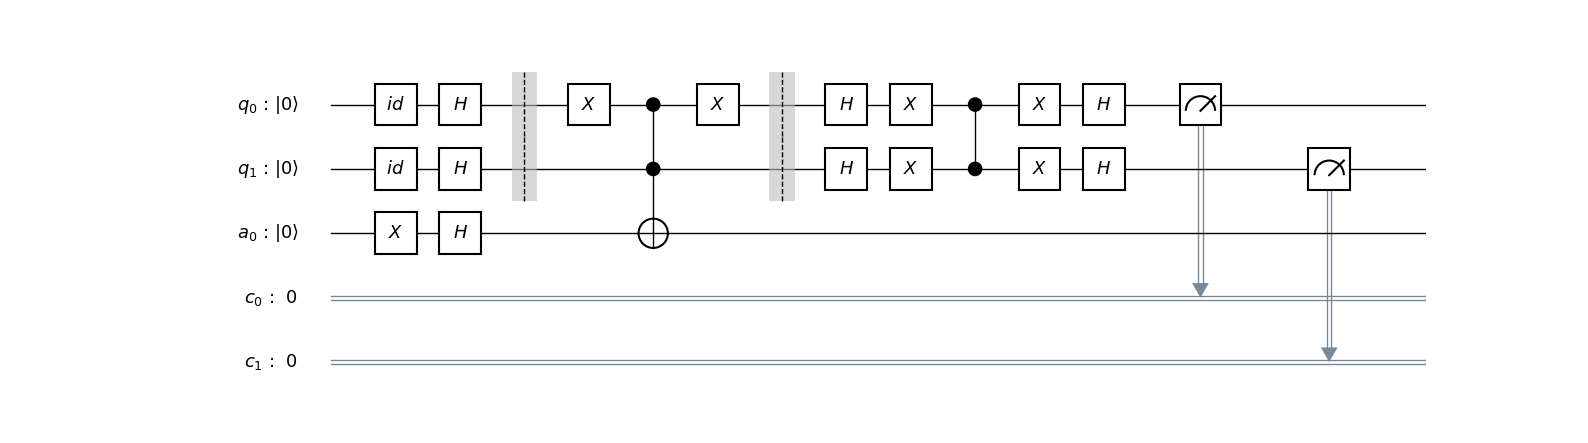
\includegraphics[trim=190 0 190 0,width=0.9\textwidth]{code/data/images/qiskit-circuit.png}
				\caption{Quantum Circuit}
			\end{figure}
		\end{column}
		\begin{column}{0.25\textwidth}  %%<--- here
			\begin{figure}
				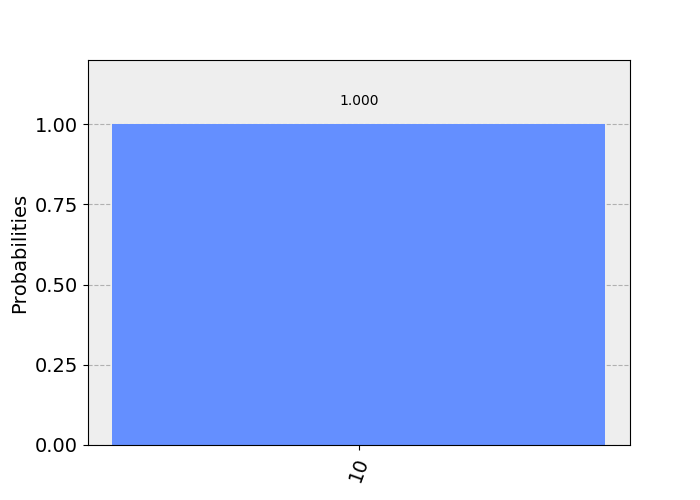
\includegraphics[width=\textwidth]{code/data/images/qiskit-histogram.png}
				\caption{Histogram}
			\end{figure}
		\end{column}
	\end{columns}
\end{frame}	

\begin{frame}[fragile]{}
	\frametitle{IBM Implementation: Quantum Experience}
	\framesubtitle{\href{https://www.research.ibm.com/ibm-q/technology/experience/}{https://www.research.ibm.com/ibm-q/technology/experience/}}
	\begin{columns}
		\begin{column}{0.75\textwidth}
			\begin{figure}
				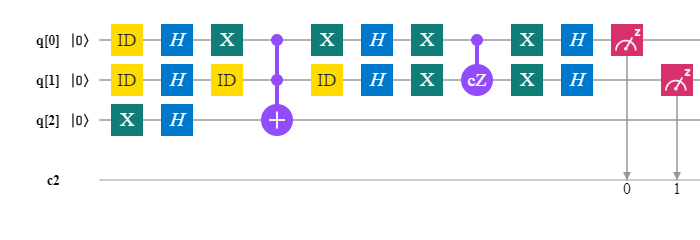
\includegraphics[trim=0 0 0 0,width=0.9\textwidth]{figures/ibm-implementation/circuit.png}
				\caption{Quantum Circuit}
			\end{figure}
		\end{column}
		\begin{column}{0.25\textwidth}  %%<--- here
			\begin{figure}
				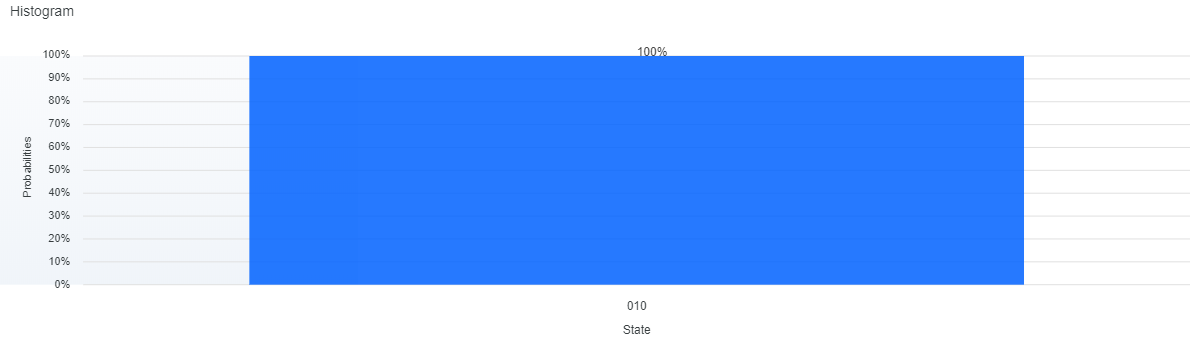
\includegraphics[width=\textwidth]{figures/ibm-implementation/histogram.png}
				\caption{Histogram}
			\end{figure}
		\end{column}
	\end{columns}
\end{frame}	
\section{References}
\nocite{
	nielsen2002quantum,
	DBLP:journals/corr/abs-1708-03684,
	van2018quantum,
	Qiskit}
\bibliographystyle{IEEEtran}
\begin{frame}
	\frametitle{References}
	\bibliography{bibliography.bib}
\end{frame}

\end{document}